\notechapter{N-20221229}{Algebraic Topology and Algebra: Products, Wedge Sums, CW Complexes, Cosets, and Surface Gluings}

\section{What this note is really doing}

This note is a working page where several threads meet: the torus as $(\mathbb R/\mathbb Z)^2$, the product $S^1\times S^1$, disjoint union and wedge sum, CW complexes, the algebra of cosets, and the square/polygon gluing pictures for surfaces.  The original page should not be compressed into a list of definitions.  Its real movement is: topology suggests quotient pictures; quotient pictures resemble congruence classes; congruence classes lead to cosets; then the topological quotient of a square returns as the torus and Klein bottle.

The top margin says that there is another intuitive understanding of
\[
  S^1\times S^1 \cong T^2.
\]
Think of a torus as a vertical circle carried around a horizontal circle.  The path traced by that moving circle is the torus.  This is not merely a picture: it is a parametrization.

\begin{figure}[H]
\centering
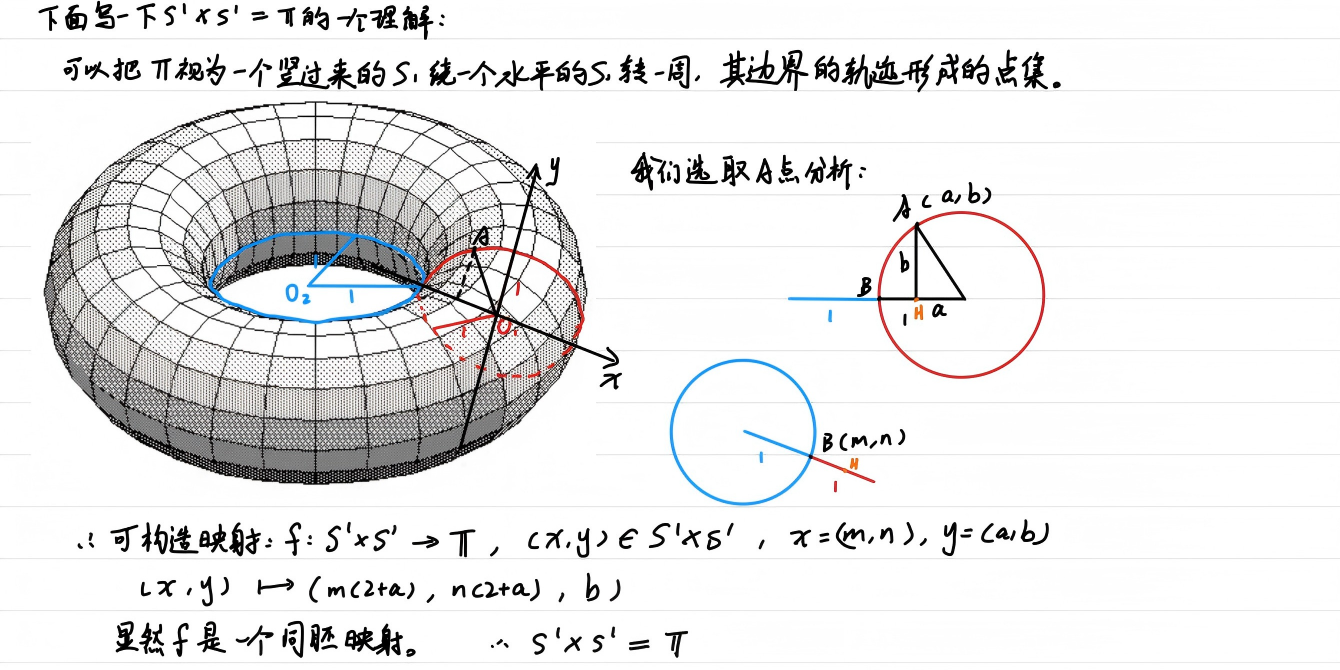
\includegraphics[width=.92\linewidth]{figures/N-20221229/01-torus-product-analysis.png}
\caption{The original visual analysis of $S^1\times S^1$: one parameter goes around the big circle, the other around the small circular fiber.}
\end{figure}

\section[The torus as a parametrized product]{\texorpdfstring{$S^1\times S^1$}{S1 x S1} as a parametrized torus}

Write a point of the first circle as an angle $\theta$, and a point of the second circle as an angle $\phi$.  For a torus with major radius $R$ and minor radius $r$, a standard parametrization is
\[
  F(\theta,\phi)=((R+r\cos\phi)\cos\theta,
  (R+r\cos\phi)\sin\theta,
  r\sin\phi).
\]
This realizes $S^1\times S^1\to T^2$.  The first angle decides where the circular cross-section is placed around the central hole; the second decides where we are on that cross-section.

The handwritten picture tries to choose a point $A$ and decompose it into two circle parameters.  That is exactly the right intuition, but the invariant statement is cleaner: the torus is the space of ordered pairs of circle-points, then realized geometrically by the map above.

\section{Disjoint union}

For topological spaces $X$ and $Y$, the disjoint union $X\amalg Y$ keeps the two spaces formally separate.  A subset $U\subseteq X\amalg Y$ is open iff
\[
  U\cap X \text{ is open in }X,
  \qquad
  U\cap Y \text{ is open in }Y.
\]
If $X$ and $Y$ are nonempty, then $X\amalg Y$ is disconnected.  Indeed, $X$ and $Y$ are both open in the disjoint union topology, disjoint, nonempty, and their union is the whole space.  This proof is more precise than the vague statement that the spaces are simply “side by side”.  The topology, not only the picture, gives the separation.

\section{Wedge sum}

The wedge sum is obtained from a disjoint union by identifying chosen basepoints:
\[
  X\vee Y=(X\amalg Y)/(x_0\sim y_0).
\]
Thus disjoint union places spaces side by side, while wedge sum fuses them at one point.  The prototype is $S^1\vee S^1$, the figure-eight space.

\begin{figure}[H]
\centering
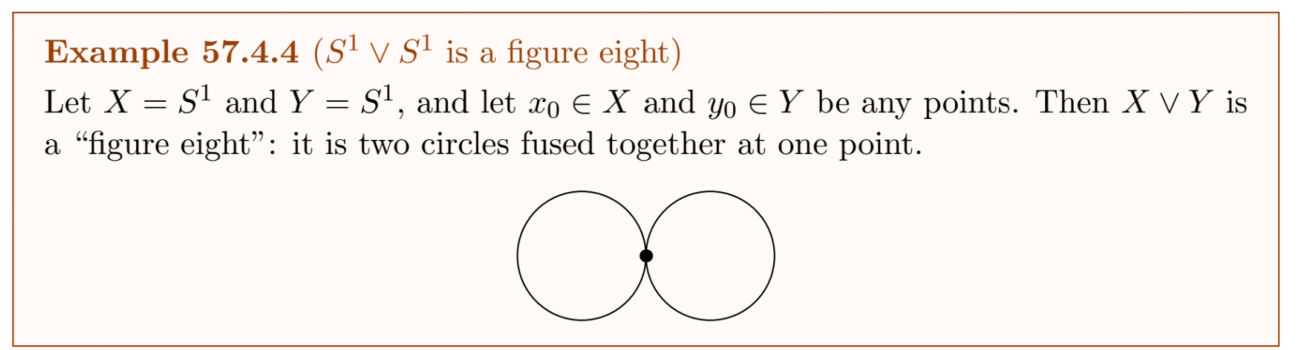
\includegraphics[width=.80\linewidth]{figures/N-20221229/02-wedge-figure-eight.png}
\caption{The wedge sum $S^1\vee S^1$ as two circles fused at one point.}
\end{figure}

This construction matters because loops in the two circles remain visibly independent.  Algebraically, the fundamental group of the figure eight is the free group on two generators.  So the picture is not a toy: it is one of the first spaces where topology produces noncommutative algebra.

\section{CW complexes: building spaces by cells}

A CW complex is built inductively.  Start with a set of $0$-cells.  Attach $1$-cells by gluing endpoints to the $0$-skeleton.  Attach $2$-cells by gluing the boundary circle of a disk to the $1$-skeleton.  Continue dimension by dimension:
\[
  X^0\subseteq X^1\subseteq X^2\subseteq\cdots.
\]
A $k$-cell is a copy of $D^k$ attached along $S^{k-1}$ by an attaching map
\[
  \varphi_\alpha:S^{k-1}_\alpha\to X^{k-1}.
\]
Informally: attach disks along their boundaries.

The note compares two CW structures on $D^2$.  One uses two $0$-cells, two $1$-cells, and one $2$-cell.  The other uses one $0$-cell, one $1$-cell whose two endpoints are glued to that point, and one $2$-cell.  Both build a disk, but the second is more economical.

\begin{figure}[H]
\centering
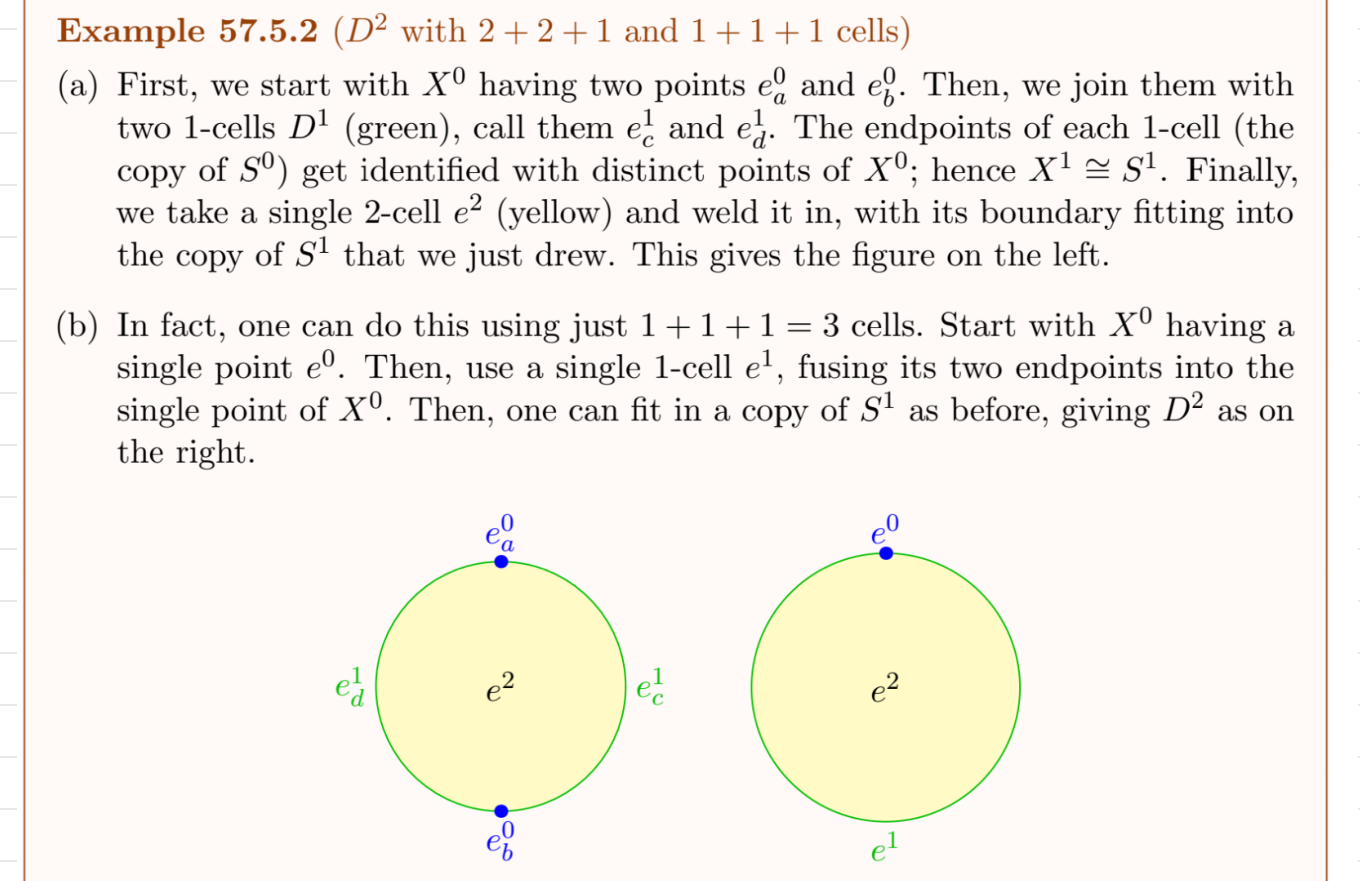
\includegraphics[width=.84\linewidth]{figures/N-20221229/03-d2-cw-cells.png}
\caption{Two CW descriptions of $D^2$: one more literal, one more economical.}
\end{figure}

The lesson is that a CW decomposition is not unique.  It is chosen because it makes later topology and algebra computable.

\section{The torus as a quotient of a square}

The torus can be formed from a square by identifying opposite edges in the same direction.  Walking off the right edge returns one at the corresponding point on the left edge; walking off the top returns one at the bottom.  Algebraically,
\[
  T^2 \cong (\mathbb R/\mathbb Z)^2 \cong S^1\times S^1.
\]
The quotient square viewpoint treats $[0,1]\times[0,1]$ as a fundamental domain for $(\mathbb R/\mathbb Z)^2$.

\begin{figure}[H]
\centering
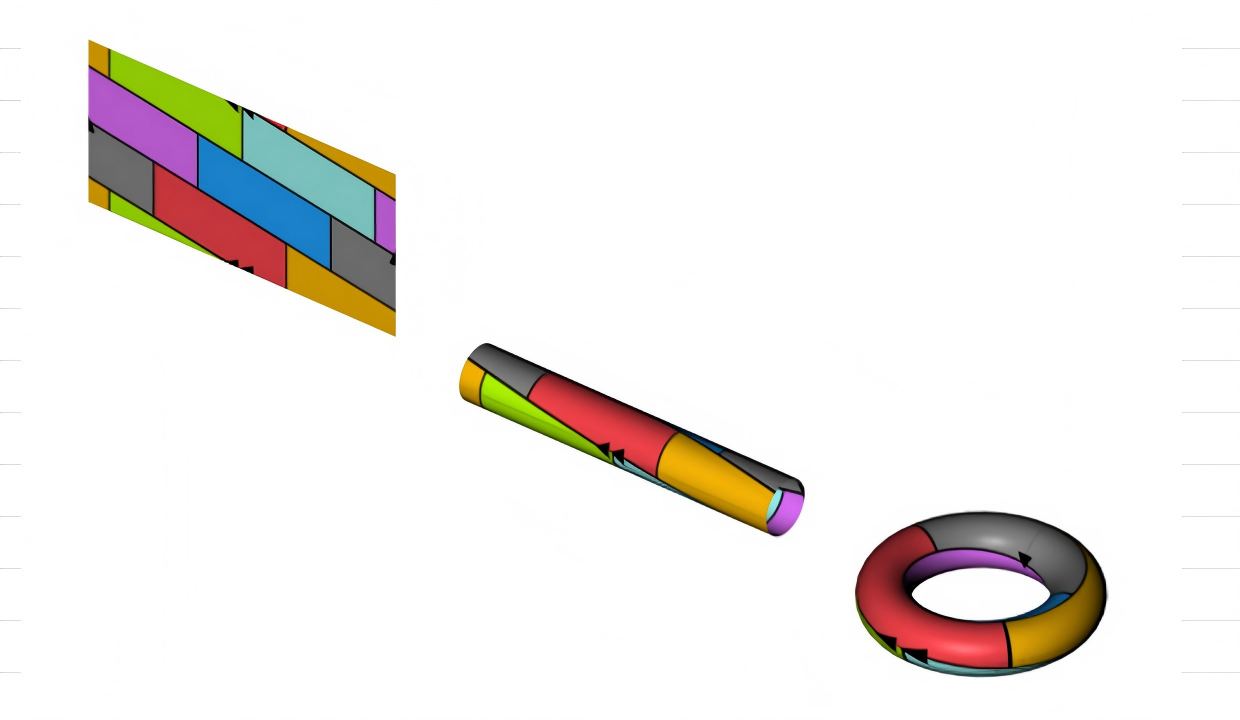
\includegraphics[width=.82\linewidth]{figures/N-20221229/04-torus-gluing-inm.png}
\caption{The quotient square/cylinder/torus picture: $(\mathbb R/\mathbb Z)^2$ as a glued square.}
\end{figure}

As a CW complex, the torus has one $0$-cell, two $1$-cells $a,b$, and one $2$-cell.  The boundary of the $2$-cell is attached along the word
\[
  aba^{-1}b^{-1}.
\]
This gives the familiar presentation
\[
  \pi_1(T^2)=\langle a,b\mid aba^{-1}b^{-1}=1\rangle\cong \mathbb Z^2.
\]
The commutativity of $\mathbb Z^2$ is encoded by the boundary word of the square.

\section{Cosets as algebraic quotients}

The algebra excerpt in the original pages is not random.  It is the algebraic analogue of quotienting.  If $H$ is a subgroup of $G$, right congruence modulo $H$ is
\[
  a\equiv_r b \pmod H
  \quad\Longleftrightarrow\quad
  ab^{-1}\in H.
\]
It is an equivalence relation.  Reflexivity uses $aa^{-1}=e\in H$; symmetry uses $(ab^{-1})^{-1}=ba^{-1}$; transitivity uses
\[
  ac^{-1}=(ab^{-1})(bc^{-1}).
\]
The equivalence class of $a$ is the right coset
\[
  Ha=\{ha:h\in H\}.
\]
The map $H\to Ha$, $h\mapsto ha$, is a bijection, so $|Ha|=|H|$.  The group $G$ is partitioned into cosets, and two cosets are either equal or disjoint.  This is exactly the algebraic version of cutting a space into equivalence classes.

This is why the note can return from cosets to $(\mathbb R/\mathbb Z)$ naturally.  Both are quotient constructions: identify things differing by a subgroup.

\section{The Klein bottle}

The Klein bottle is built like the torus, except one pair of edges is identified in the opposite direction.  If one first glues a pair of edges, one gets a cylinder.  But gluing the resulting boundary circles in opposite directions cannot be embedded in ordinary three-dimensional space without self-intersection.  The usual picture in $\mathbb R^3$ is therefore an immersion, not a faithful embedding.

\begin{figure}[H]
\centering
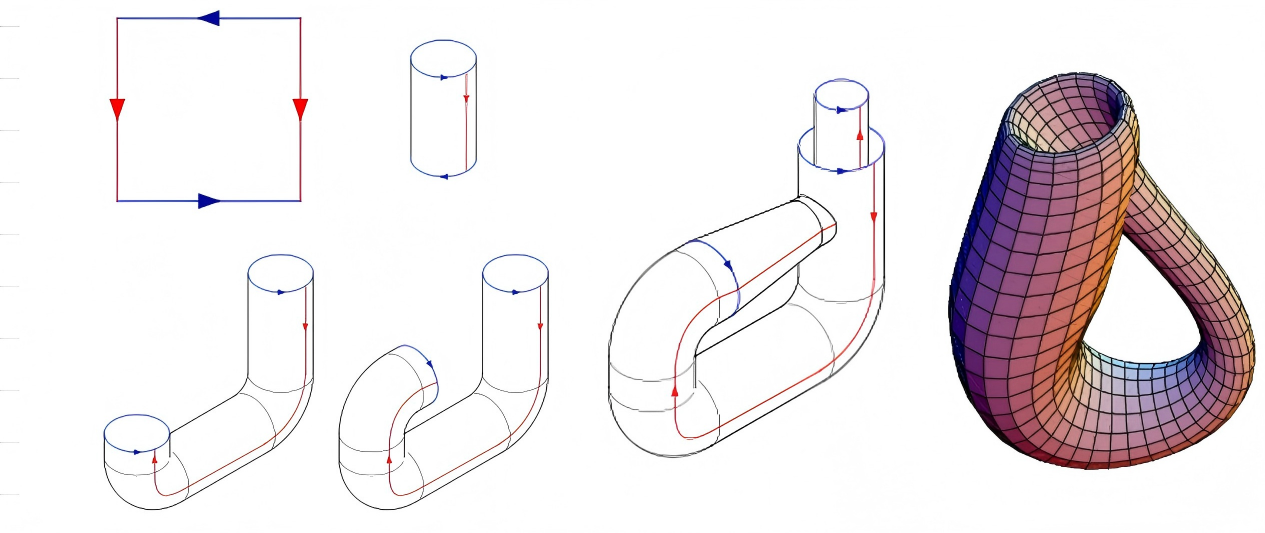
\includegraphics[width=.86\linewidth]{figures/N-20221229/05-klein-bottle-gluing.png}
\caption{The Klein bottle: one edge identification is reversed, so the usual 3D picture self-intersects.}
\end{figure}

As a CW complex, the Klein bottle again has one $0$-cell, two $1$-cells, and one $2$-cell, but the attaching word changes.  A common presentation is
\[
  \pi_1(K)=\langle a,b\mid aba^{-1}=b^{-1}\rangle.
\]
The relation says that going around one direction reverses the other.  Thus the torus and Klein bottle have the same cell counts but different attaching words, and this difference controls orientability and fundamental group.

\section{Polygon schemata for surfaces}

The last figure records polygon schemata for surfaces.  A polygon with labelled, oriented boundary edges can be glued according to those labels.  The resulting quotient is a surface.  For example, the torus corresponds to
\[
  aba^{-1}b^{-1},
\]
while an orientable surface of genus $g$ has a boundary word of the form
\[
  a_1b_1a_1^{-1}b_1^{-1}\cdots a_gb_ga_g^{-1}b_g^{-1}.
\]

\begin{figure}[H]
\centering
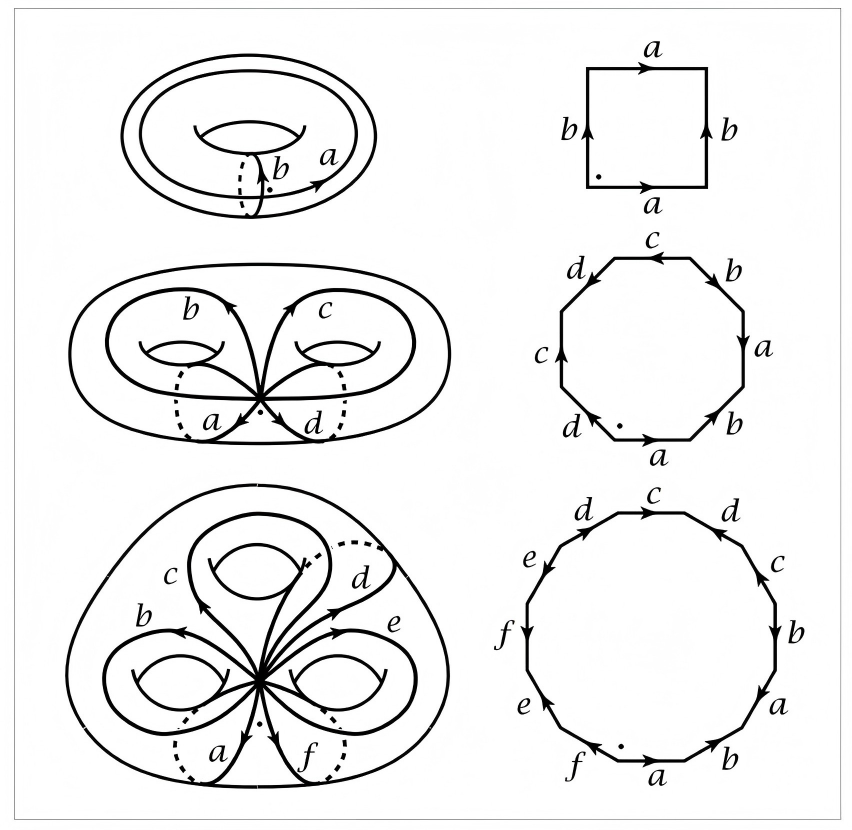
\includegraphics[width=.70\linewidth]{figures/N-20221229/06-surface-polygon-schema.png}
\caption{Polygon schemata and surface gluings: topology encoded by labelled boundary words.}
\end{figure}

The handwritten comment says these diagrams took a long time to understand.  That is exactly right.  The picture compresses several ideas: cut a surface into a polygon, label the boundary, glue equal labels, and read the labels as algebraic generators and relations.

\section{Projective spaces as quotient spaces}

The section title also mentions real and complex projective spaces.  They fit the same quotient philosophy.  Real projective space is
\[
  \mathbb{RP}^n=S^n/(x\sim -x),
\]
the space of lines through the origin in $\mathbb R^{n+1}$.  Complex projective space is the space of complex lines through the origin in $\mathbb C^{n+1}$, equivalently
\[
  \mathbb{CP}^n=S^{2n+1}/S^1.
\]
A useful CW fact is that $\mathbb{RP}^n$ has one cell in each dimension $0,1,\ldots,n$, while $\mathbb{CP}^n$ has one cell in each even real dimension $0,2,4,\ldots,2n$.


\section{Cellular boundary words and fundamental groups}

The attaching word of the two-cell is not a decorative label.  For the torus, the word
\[
  aba^{-1}b^{-1}
\]
becomes the relation saying that \(a\) and \(b\) commute.  For the Klein bottle, the twist changes the relation to one of the form
\[
  aba^{-1}=b^{-1}.
\]
Thus two spaces can have the same numbers of cells but different topology because the attaching maps differ.

\section{Why polygon schemata are efficient}

A labelled polygon schema compresses a surface into boundary data.  The labels record which edges are glued, and the arrows record orientation.  Once this is understood, the diagram becomes an algebraic object: reading around the boundary gives a word in generators and inverses.

This is the reason algebraic topology can turn pictures into group presentations and chain complexes.

\section{Further context}

The repaired version of this note should be read as one continuous story.  First, $S^1\times S^1$ parametrizes the torus.  Second, a square with opposite sides identified gives the same torus as a quotient.  Third, disjoint union and wedge sum explain how spaces can be combined before quotienting.  Fourth, CW complexes systematize this by attaching cells.  Fifth, cosets provide the algebraic analogue of quotienting.  Finally, torus, Klein bottle, and polygon schemata show that a whole surface can be encoded by a boundary word.

The central lesson is that algebraic topology is not simply topology plus algebra added later.  The topology is already algebraic as soon as we record how pieces are glued: arrows, labels, words, equivalence classes, and quotient maps are the bridge.


\paragraph{Expanded synthesis.}
For this chapter, the elementary material should be read as a study of what remains invariant when coordinates change. The earlier sections (`What this note is really doing`, `$S^1\times S^1$ as a parametrized torus`, `Disjoint union`, `Wedge sum`, `CW complexes: building spaces by cells`) compute with arrays, bases, pivots, determinants, or eigenvectors; the deeper object is a linear map together with the spaces it acts on. A matrix is a representation of that map after bases have been chosen. This is why formulas such as
\[
  A' = P^{-1}AP,\qquad \widetilde A = T^{-1}AS
\]
are not cosmetic: they distinguish an intrinsic morphism from a coordinate description.

The structural hierarchy is as follows. Kernels record what a map forgets, images record what it reaches, cokernels record obstructions to solvability, and quotients record information after an equivalence has been imposed. Determinants act on the top exterior power and therefore measure oriented volume; traces are invariant under cyclic rearrangement and become characters in representation theory; adjoints depend on an inner product and lead to self-adjoint spectral theory.

A useful way to return to the computations is to ask, for every formula, which invariant it is measuring. Row reduction measures rank and kernel; diagonalization measures decomposition into invariant subspaces; Gram--Schmidt measures orthogonal projection; positive definiteness measures ellipsoid geometry; tensor notation measures how components transform. The elementary methods are therefore the finite-dimensional laboratory in which duality, quotienting, functoriality, and spectral decomposition can be seen clearly.
